\chapter{Parallel DNS of a turbulent channel flow}


\section{Problem definition}
\pagestyle{headings}

Before moving to what has been done in this thesis I wish to briefly discuss the setup of our channel flow and the equations used to solve the problem.

\begin{figure}[h]
\centering
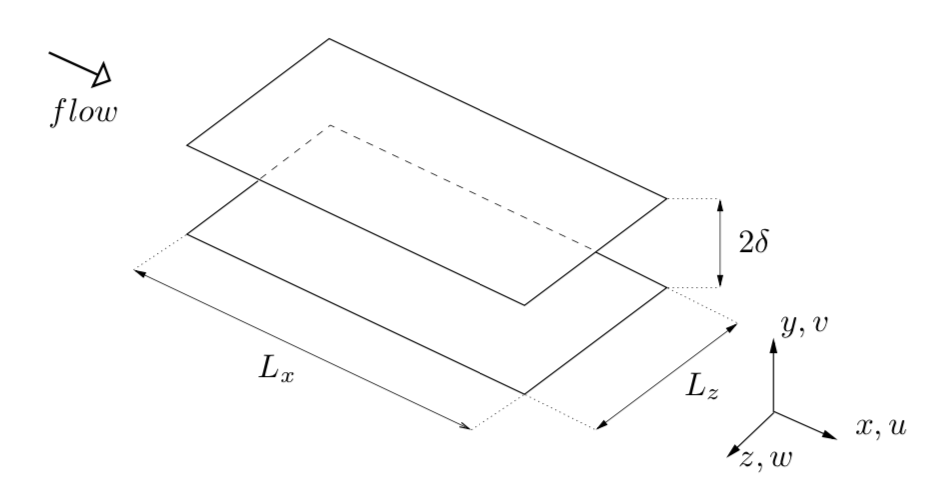
\includegraphics[width=0.8\textwidth]{grafici/sketch_dominio}
\caption{Domain of interest}
\label{sketch_dominio}
\end{figure}

We have the domain sketched in figure~\ref{sketch_dominio} where the $x$ and $z$ coordinates denote the streamwise and spanwise directions of the flow, while the $y$ coordinate is the wall normal ones.
Along these three dimensions we have $u,v$ and $w$ components of velocity.

The flow is assumed to be periodic in the streamwise and spanwise directions. The lower wall is at position $y_l$ and the upper wall at position $y_u$. The reference length $\delta$ is taken to be one half of the channel height.
Once an appropriate reference velocity is chosen, we can define the Reynolds number as:
\[
Re = \frac{U\delta}{\nu}
\]
where $\nu$ is the kinematic viscosity of the fluid.

According to our geometry and the assumption of incompressible flow, we can express the behavior of the flow through the mass conservation law:
\begin{equation}
\frac{\partial u}{\partial x} + \frac{\partial v}{\partial y} + \frac{\partial w}{\partial z} = 0
\label{mass:cons}
\end{equation}
 and the Navier-Stokes equations, which in a dimensionless form states:
\begin{subequations}
\label{eqn:ns}
\begin{align}
\frac{\partial u}{\partial t} + u\frac{\partial u}{\partial x} + v\frac{\partial u}{\partial y} + w\frac{\partial u}{\partial z} &= 
- \frac{\partial p}{\partial x} + \frac{1}{Re} \nabla^{2}u  \label{eqn:ns:1}\\
\frac{\partial v}{\partial t} + u\frac{\partial v}{\partial x} + v\frac{\partial v}{\partial y} + w\frac{\partial v}{\partial z} &= 
- \frac{\partial p}{\partial y} + \frac{1}{Re}\nabla^{2}v \label{eqn:ns:2}\\
\frac{\partial w}{\partial t} + u\frac{\partial w}{\partial x} + v\frac{\partial w}{\partial y} + w\frac{\partial w}{\partial z} &= 
- \frac{\partial p}{\partial z} + \frac{1}{Re}\nabla^{2}w \label{eqn:ns:3}
\end{align}
\end{subequations}
The differential problem is closed when initial conditions for all the fluid variables are specified, and suitable boundary conditions are chosen. At the walls the no-slip condition are imposed.








\section{Governing equations}
The numerical method does not rely on the equations~\eqref{eqn:ns}, instead it solves the wall-normal velocity and the wall-normal vorticity equations, recovering, at the end of the the solution, the three velocity components.\\
\subsection{Wall normal vorticity equation}
Defining the wall-normal component of the vorticity vector as:
\[
\eta = \frac{\partial u}{\partial z} - \frac{\partial w}{\partial x}
\]
which, in Fourier space, holds:
\[
\hat{\eta} = i\beta \hat{u} - i \alpha \hat{w}
\] 
with the hat indicating Fourier-transformed quantities, $i$ the imaginary part, $\alpha$ and $\beta$ the streamwise and spanwise wave numbers;  allows to write a one-dimensional second-order evolutive equation for $\hat{\eta}$ which does not involve pressure, as proposed in \cite{kim_moin_moser}.

Taking the y-component of the curl of the momentum equation we obtain:
\begin{equation}
\label{curl:momentum:y}
\frac{\partial \hat{\eta}}{\partial t}  = \frac{1}{Re}  \big( D_{2}(\hat{\eta}) - k^{2} \hat{\eta} \big) + i \beta \widehat{HU} -i \alpha \widehat{HW}
\end{equation}
where $D_{2}$ is the second derivative in the wall-normal direction, $k^{2}$ is the sum of $\alpha$ and $\beta$, and the nonlinear terms are defined as:

\begin{subequations}
\label{nonlinear:terms}
\begin{align}
\widehat{HU} &= i \alpha \widehat{uu} + D_{1} \widehat{uv} + i \beta \widehat{uw}\\ 
\widehat{HV} &= i \alpha \widehat{uv} + D_{1} \widehat{vv} + i \beta \widehat{vw}\\
\widehat{HW} &= i \alpha \widehat{uw} + D_{1} \widehat{vw} + i \beta \widehat{ww}.
\end{align}
\end{subequations}

To solve the equation \eqref{curl:momentum:y} we must set suitable initial conditions for $\hat{\eta}$. Such initial conditions are computed using the initial velocity field and the definition of $\eta$ itself.
Turning such conditions into frequency domain is straightforward and satisfy the periodic boundary conditions. Finally, the \emph{no-slip} condition for velocity vector enforce the condition at the walls, which, simply, translate in $\hat{\eta}=0$ at $y=y_{l}$ and $y=y_{u}$.


\subsection{Wall normal velocity equation}
An equation for the wall-normal velocity component $\hat{v}$, which does not involve pressure, is derived in \cite{kim_moin_moser}, by summing the equation \eqref{eqn:ns:1} derived two times w.r.t. $x$ and $y$, and \eqref{eqn:ns:3} derived two times w.r.t. $y$ and $z$, then subtracting \eqref{eqn:ns:2} derived w.r.t. $x$ and $x$ and substracting once again after derivation w.r.t. $z$ and $z$.
Further simplifications are invoked through the equation \eqref{mass:cons}, which lead to the following fourth-order evolutive equation for $\hat{v}$, which is the so called wall-normal velocity equation:
\begin{multline}
\label{normal:velocity}
\frac{\partial}{\partial t} \big( D_{2}(\hat{v}) - k^{2} \hat{v} \big) = \frac{1}{Re} \big( D_{4}(\hat{v}) - 2k^{2} D_{2}(\hat{v}) + k^{4} \hat{v} \big) \\
	-k^{2} \widehat{HV} - D_{1} \big(  i \alpha \widehat{HU} + i \beta \widehat{HW} \big).
\end{multline}
To solve such equation we have to enforce initial conditions on $\hat{v}$.\\
According to Fourier expansions, the periodic boundary conditions in the homogeneous directions are automatically satisfied, whereas the no-slip condition for the velocity vector immediately translates in $\hat{v} = 0$ to be imposed at the two walls.\\
The two remaining conditions for the fourth-order equation \eqref{normal:velocity} comes from the continuity equation \eqref{mass:cons}, written at the vertical edges of the domain, $y= y_{l}$ and $y=y_{u}$.


\subsection{Velocity components in the homogeneous directions and mean flow}
As reported before, once the two preceding equations are solved, we can use them to recover the velocity components in the homogeneous directions.\par
Assuming the non-linear terms \eqref{nonlinear:terms} known, as is the case when such terms are treated explicitly in the time discretization, the equations \eqref{curl:momentum:y} and \eqref{normal:velocity} become uncoupled and, after proper time discretization, can be solved for advancing the solution by one time step, provided the nonlinear terms \eqref{nonlinear:terms} and their spatial derivatives can be calculated.
To this aim, one needs to know how to compute $\hat{u}$ and $\hat{w}$ at a given time starting with the knowledge of $\hat{v}$ and $\hat{\eta}$. \\
By using the definition \eqref{curl:momentum:y} of $\hat{\eta}$ and the continuity equation \eqref{mass:cons} written in Fourier space, a 2 $\times$ 2 algebraic system can be written for the unknowns $\hat{u}$ and $\hat{w}$; its analytical solution read:

\begin{equation}
\begin{cases}
\label{uw:eq}
\hat{u} &= \dfrac{1}{k^{2}} ( i \alpha D_{1}(\hat{v} ) - i \beta \hat{\eta})\\\\
\hat{w} &= \dfrac{1}{k^{2}} (i \alpha \hat{\eta} + i \beta D_{1}(\hat{v}))
\end{cases}
\end{equation}
For $k^{2}=0$ the system of equation \eqref{uw:eq} is singular. \par
The present method therefore enjoys its highest computational efficiency only when Fourier discretization is used in the homogeneous directions.
\par
Since the previous system of equations \eqref{uw:eq} has been obtained starting from equations \eqref{curl:momentum:y} and \eqref{normal:velocity} the solutions are sensible to homogeneous spatial derivatives through the wave numbers. \par
Let us introduce a plane-average operator defined as:
\begin{equation}
\tilde{f} = \frac{1}{L_{x}} \frac{1}{L_{z}} \int_{0}^{L_{x}} \int_{0}^{L_{z}} f \,dx \,dz.
\end{equation}
If we apply such operator to our velocity components vector $\mathbf{V}$, it turns out that $\mathbf{V}(x,y,z,t)~=~\mathbf{\widetilde{V}}(y,t) $. According to this, our velocity components are function of time and wall-normal coordinate only. In Fourier domain this behavior is denoted by the absence of the wave numbers, so for $k^{2}=0$. \par

In agreement with our reference system, where the $x$ axis is aligned with the mean flow, the temporal average of $\tilde{u}$ will denote the mean velocity profile, whereas the temporal average of $\tilde{w}=0$ throughout the channel. \\
Anyway $\tilde{w}$ can be different from zero at different time and distance from the wall. \par

Finally, applying the plane-average operator to the components of the momentum equation let us compute the $\tilde{u}$ and $\tilde{w}$:
\begin{subequations}
\begin{align}
\frac{\partial{ \tilde{u}}}{\partial t} &=  \frac{1}{Re} D_{2} ( \tilde{u}) - D_{1}( \widetilde{uv}) + f_{x} \\
\frac{\partial{ \tilde{w}}}{\partial t} &= \frac{1}{Re} D_{2}( \tilde{w}) - D_{1} ( \widetilde{vw}) + f_{z}
\end{align}
\end{subequations}

 In these expressions, $f_{x}$ and $f_{z}$ are the forcing terms needed to force the flow through the channel against the viscous resistence of the fluid. For the streamwise direction, $f_{x}$ can be an imposed mean pressure gradient, and in the simulation the flow rate through the channel will oscillate in time around its mean value. $f_{x}$ can also be a time-dependent spatially uniform pressure gradient, that has to be chosen in such a way that the flow rate remains constant in time. The same distinction applies to the spanwise forcing term $f_{z}$: in this case however the imposed mean pressure gradient or the imposed mean flow rate is zero, while the other quantity will be zero only after time average.\\
\par
\par
What has been shown in this chapter is intended just to be a brief discussion. Further informations are available in~\cite[1-3]{cpl:presentazione}.

